\section{Snap!}
\label{solution SNAP}
Comme expliqués précédemment, nous sommes partis d'un projet existant, Snap! BYOB, pour l'environnement de programmation. Ce projet a pour but de fournir une interface et un environnement supportant la programmation par bloc. Ce projet ne s'inscrit pas dans le cadre d'un apprentissage scolaire ou guidé. Il a donc fallu adapter le projet pour une utilisation plus scolaire. Nous allons expliquer dans cette partie les différentes adaptations que nous avons apportées au projet d'origine et pourquoi elles sont nécessaire pour remplir nos objectifs.\\

Dans les adaptations opérées, nous retiendrons : une simplification de l'interface, la sauvegarde sur les serveurs du projet courant, une différenciation de rôle pour le professeur par rapport au public cible, une amélioration de la traduction en français, le masquage des scripts.

\begin{figure}[]
  \begin{center}
  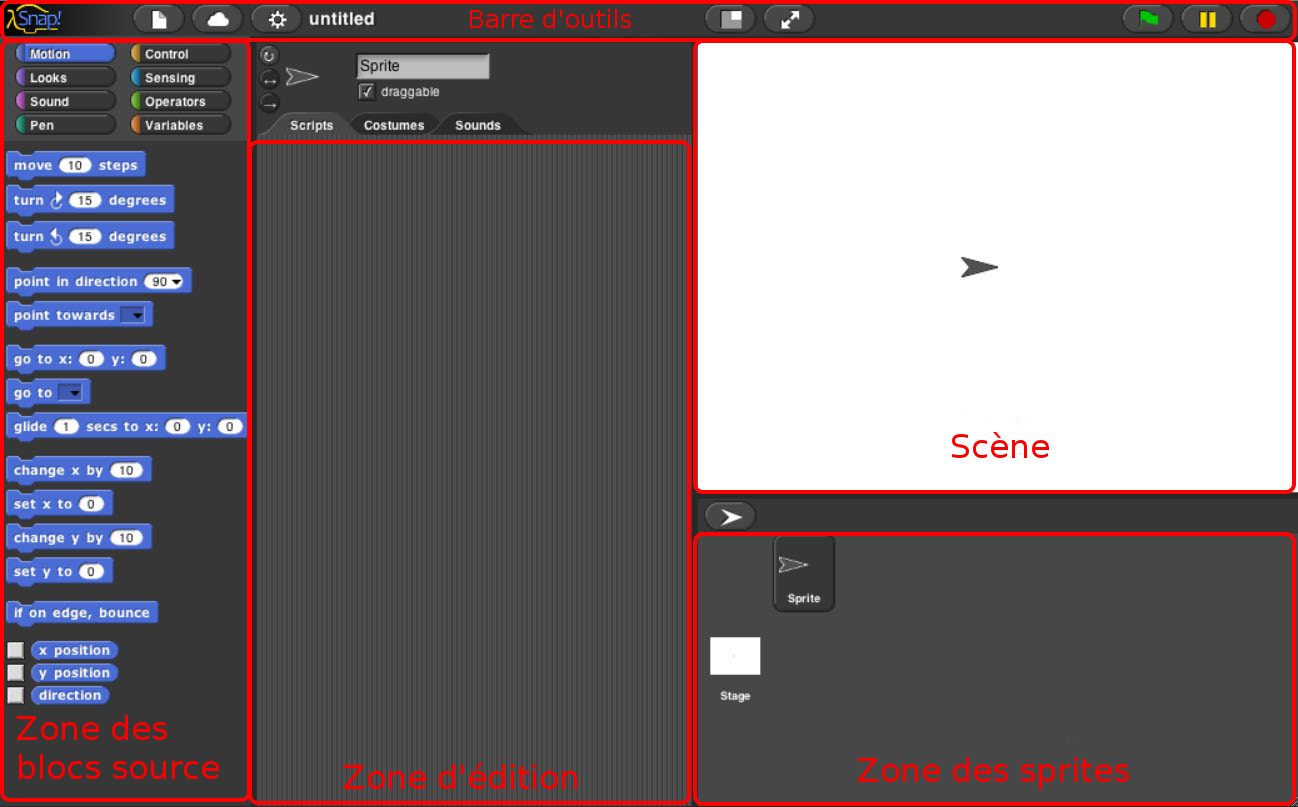
\includegraphics[width=\textwidth]{content/7-solution/2-snap/images/interface}
        \caption{Délimitation des zones de l'interface Snap!}
    \label{fig:snap interface}
  \end{center}
\end{figure}

\subsection{L'interface}
\label{interface}
Comme expliqué précédemment le projet original n'avait pas une vocation didactique de groupe et avait un publique cible plus large que le notre. Dans cette idée, il y avait des menus pour des fonctionnalités de gestion de l'ordonnanceur, option d'affichage, paramètres d'éditions, etc. Il est évident que ces fonctionnalités ne sont pas utiles pour notre public. De plus vu l'âge de notre public toutes distractions qui peuvent être évitées améliorent sensiblement l'attention de ces derniers.

Dans cette optique, nous avons opéré un nettoyage en profondeur de l'interface dans l'optique de laisser uniquement les menus utiles. Toutefois comme il est discuté dans les rôles \ref{role}, il est intéressant de ne pas simplement les effacer, mais bien de les masquer.\\

Une autre adaptation de l'interface réalisée est l'ajout d'un menu pour les interactions avec notre plateforme web. Ce menu contient des boutons tel que : "sauvegarder sur le serveur" pour enregistrer leur travail sur la plateforme; "description" qui permet de retrouver le résumé introductif de la mission; "retour à la liste des missions" qui demande a sauver le travail puis renvoie vers la page listant les missions sur le site web.

\subsection{Les rôles}
\label{role}
Dans l'optique de fournir une interface épurée pour les étudiants comme expliqués dans la section \ref{interface}. Il était nécessaire d'enlever des parties de l'interface non pertinente. Toutefois, ces options inutiles aux étudiants peuvent l'être pour les professeurs, mais également pour une mission en "monde ouvert". Il est donc utile de ne pas dédoubler les interfaces, mais bien d'avoir une interface modulaire suivant son utilisation. \\

Pour différencier les utilisations de l'interface, nous avons ajouté la notion de rôles. Nous avons défini deux rôles: étudiant et professeur. Grâce à cela, quand les étudiants ouvre un projet, Snap! est lancé avec le rôle étudiant ce qui permet de ne pas afficher les options superflues. Quand c'est un professeur qui souhaite modifier une mission ou en créer une nouvelle, RSNAP lance Snap! avec le rôle professeur ce qui permet d'avoir accès aux fonctions avancées de Snap!.\\

Ces rôles permettent également la gestion du masquage de script. En effet, il est intéressant qu'un professeur puisse masquer des blocs, mais cela ne sert à rien si les étudiants peuvent les réafficher.

\subsection{Masquer les scripts}
Il a été nécessaire pour la création des missions de cacher des blocs aux étudiants. Par exemple, la partie de vérification du code de l'étudiant ou encore le code de l'environnement de la mission ne doivent pas apparaître pour les étudiants. 

Une possibilité de cacher des blocs existait déjà dans la zone des blocs sources (voir l'interface sur la figure \ref{fig:snap interface}) de l'interface pour que tous les blocs n'apparaissent pas comme on peut le voir sur la figure \ref{fig:cacher}. Nous avons étendu cette fonction pour pouvoir également cacher des blocs ou des scripts dans la partie d'édition.

Il a également fallu ajouter cette information dans la sauvegarde du projet. Ceci a été réalisé grâce à la balise \texttt{hidden} dans le XML. Cette balise n'est présente que si le bloc doit être caché pour limiter les ajouts au document de sauvegarde.\\

Cette fonctionnalité pouvant être intéressante pour le projet original, elle a été proposée dans une \texttt{pull request}. Les responsables de Snap! ont été très intéressé par cette fonctionnalité qui est toujours en cours d'étude.
\begin{figure}[]
  \begin{center}
    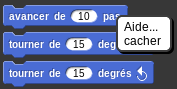
\includegraphics[scale=0.5]{content/7-solution/2-snap/images/cacher}
    \caption{Option pour cacher la définition d'un bloc}
    \label{fig:cacher}
  \end{center}
\end{figure}

\subsection{Traduction}
Le caractère francophone de ce travail est une part importante dans sa différenciation par rapport aux autres initiatives similaires introduites dans la section \ref{travail associé}. L'application était déjà traduite partiellement en français, mais une large majorité des traductions étaient incomplètes, inexistantes ou erronées. Une partie du travail a donc été de finir et amélioré la traduction de l'application. La traduction de l'application se divise en deux parties, la partie interface et la partie aident. Pour ce travail ont été développés des outils de traduction d'aide automatisé. Ces outils ont été développés, car des aides en français existaient déjà dans le projet SCRATCH. Il était donc plus efficace d'avoir un outil de traduction automatique que de retraduire manuellement les aides.

Cette partie a été proposée au projet original de Snap! et acceptée, mais ne sera intégré qu'après quelques aménagements. Elle est donc actuellement acceptée, mais en attente.

\subsection{Sauvegarde sur le serveur}
Comme il était nécessaire d'interfacé l'environnement de programmation avec un site web, nous avons du reimplementer certaine fonctionnalité d'import-export.\\

Il était nécessaire de disposer d'un fichier XML pour le sauvegarder sur les serveurs. Des fonctions existantes ont été adaptées pour permettre d'avoir ce fichier et de pouvoir l'envoyer sur l'adresse internet désirée.

